Facciamo un ripasso dei numeri complessi, perche' come vedremo saranno fondamentali per rappresentare i segnali che studieremo.

\section{Rappresentazione cartesiana}
La rappresentazione cartesiana di un numero complesso generale e':
\begin{equation}
    z = x + i y
\end{equation}
Dove $x  \in \mathbb R$, $x  \in \mathbb R$ ed $i = j = \sqrt{-1}$ ed e' detta unita' immaginaria.
Riportando queste informazioni su un piano cartesiano di cui l'asse delle Y appartiene ai numeri immaginari e l'asse delle X appartiene ai numeri reali otteniamo:

\begin{figure}[ht!]
    \centering
    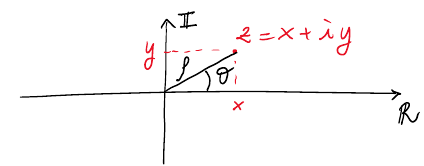
\includegraphics{immagini/lez2/rappCartesiana.jpg}
\end{figure}

\section{Rappresentazione Polare}
Oltre alla rappresentazione cartesiana esiste anche la rappresentazione polare, che punta a rappresentare il numero complesso utilizzando l'angolo che si forma tra l'asse x e la semiretta che rappresenta il numero complesso.

E la rappresentazione polare e':
\begin{equation}
    z = \rho [\cos \theta + i \sin \theta]
\end{equation}
Ci sono due componenti fondamentali in questa rappresentazione:
\begin{itemize}
    \item Modulo: $\rho$
    \item Fase: $\theta$
\end{itemize}

Si puo' passare tra le due rappresentazioni seguendo queste formule, ricordando che la rappresentazione cartesiana e': $z = x + iy$

\begin{table}[ht!]
    \centering
    \begin{tabular}{c|c}
        Rapp. Cartesiana & Rapp. Polare  \\
        \hline
        $x = \rho \cos \theta$ & $\rho = \sqrt{{x^2} + {y^2}}$\\
        $y = \rho \sin \theta$ & $\theta = \arctan \frac{y}{x}$\\
    \end{tabular}
    \caption{Passare da rappresentazione cartesiana a polare}
    \label{table:cambioRappresentazione}
\end{table}

\subsection{Esercizio}
Proviamo ora a fare un esercizio, dobbiamo rappresentare in forma polare il seguente numero immaginario espresso in forma cartesiana:
\begin{equation}
    z = -2 + i \cdot 3
\end{equation}

Cominciamo calcolando il modulo applicando semplicemente la formula vista in tabella \ref{table:cambioRappresentazione}:
\begin{equation}
    \rho = \sqrt{{-2^2} + {3^2}} = \sqrt{13}
\end{equation}

Successivamente calcoliamo la fase, sempre applicando la formula vista in tabella \ref{table:cambioRappresentazione}:
\begin{equation}
    \theta = \arctan - \frac{3}{2}
\end{equation}

Sulla fase abbiamo un problema, in quanto se dovessimo fare $\arctan - \frac{3}{2}$ alla calcolatrice ci risulterebbe $-56.3^{\circ}$, che non ha senso a prima vista in quanto negativo.
Spieghiamo questa cosa in quanto la calcolatrice ragiona solo nei quadranti 1 e 4 del piano cartesiano, quindi per sistemare questo problema dobbiamo sommare (o sottrarre) $180^{\circ}$ all'angolo che abbiamo trovato, ottenendo quindi: $123.7^{\circ}$.

\section{Coniugato Complesso}
Ogni numero immaginario ha un suo coniugato complesso, che ha lo stesso modulo e fase con segno invertito rispetto al numero immaginario di partenza.

\begin{equation}
    z = x + i y \rightarrow z^* = x - i y
\end{equation}

Graficamente otteniamo un punto ribaltato rispetto all'asse x:

\begin{figure}[ht!]
    \centering
    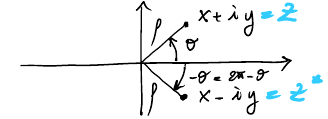
\includegraphics{immagini/lez2/coniugatoComplesso.jpg}
    \caption{Coniugato Complesso}
    \label{fig:coniugatoComplesso}
\end{figure}

\subsection{Operazioni}
Vediamo ora le operazioni con tra un numero immaginario ed il suo complesso.

Somma:
\begin{equation}
    z + z^* = x + x = 2x
\end{equation}
La somma di un numero complesso ed il suo coniugato e' uguale a due volte la sua parte reale.

Prodotto:
\begin{equation}
    z + z^* = (x + i y) \cdot (x - i y) = x^2 - i y x + i y x - i^2 y^2 = x^2 + y^2 = \rho^2
\end{equation}
Notiamo che $i^2 = (\sqrt{-1})^2 = -1$.

\section{Teorema fondamentale dell'algebra}
Data un equazione polinomiale di grado $N \ge 1$
\begin{equation}
    a_n z^n + a_{n-1} z ^ {n-1} + \mbox{...} a_1 z + a_0 = 0
\end{equation}
Ammette sempre e solo N soluzioni (radici) in $\mathbb C$.
Inoltre se $a_k \in \mathbb R$ (sono numeri reali) le soluzioni sono reali o complesse coniugate. Questa cosa introduce una simmetria, sappiamo che se i termini del polinomio sono reali non avremo mai un complesso da solo ma sara' sempre accompagnato dal suo coniugato ed e' una cosa che servira' successivamente.

\section{Formula di Eulero}
Esprimo prima cos, sin e l'esponenziale in serie:
\begin{equation}\begin{split}
    \cos& \theta = 1 - \frac{1}{2!} \theta^2 + \frac{1}{4!} \theta^4 - \frac{1}{6!} \theta^6 \mbox{...} \\
    \sin& \theta = \theta - \frac{1}{3!} \theta^3 + \frac{1}{5!} \theta^5 - \frac{1}{7!} \theta^7 \mbox{...} \\
    e^{\theta}& = 1 + \theta + \frac{\theta^2}{2!} + \frac{\theta^3}{3!} + \frac{\theta^4}{4!} + \mbox{...}
\end{split}\end{equation}

Eulero nota che se cerchiamo di calcolare l'esponenziale in serie moltiplicando l'esponente per i, il fattore i e' presente solo nei termini dispari, se sviluppiamo le potenze. 

\begin{equation}\begin{split}
    e^{i \theta}& = 1 + (i \theta) + \frac{(i \theta)^2}{2!} + \frac{(i \theta)^3}{3!} + \frac{(i \theta)^4}{4!} + \mbox{...} \\
    & = 1 + i \theta - \frac{\theta^2}{2!} - \frac{i \theta^3}{3!} + \frac{\theta^4}{4!} + \mbox{...}
\end{split}\end{equation}

Da questa considerazione troviamo la formula di Eulero :
\begin{equation}
    e^{i \theta} = \cos \theta + i \sin \theta
\end{equation}

\begin{figure}[ht!]
    \centering
    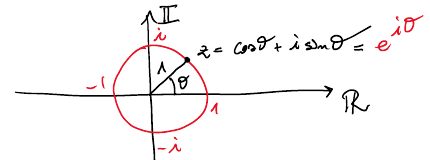
\includegraphics{immagini/lez2/formulaEulero.jpg}
    \caption{Rappresentazione su cerchio unitario}
    \label{fig:euleroGrafico}
\end{figure}

\subsection{Formule di Eulero inverse}
Esistono delle formule di Eulero con cui trovare sin e cos a partire dall'esponenziale:

\begin{equation}\begin{split}
    \cos \theta & = \frac{e^{i \theta} + e^{-i \theta}}{2}\\
    \sin \theta & = \frac{e^{i \theta} - e^{-i \theta}}{2i}
\end{split}\end{equation}